\documentclass[12pt]{article}
\usepackage{amsmath}
\usepackage{fancyhdr}
\usepackage{graphicx} 
\usepackage{tikz}
\usepackage{pgfplots}
\usetikzlibrary{shapes,backgrounds}
\usepackage[margin=1in]{geometry}

\pagestyle{fancy}
\lhead{CSCI 6550}
\chead{\textbf{Week 3 Assignment Report}}
\rhead{Eric Miller}

\begin{document}
\subsection*{Introduction}
For the third week, I worked on alpha-beta pruning for the minimax algorithm. Once this was completed, I updated the board hash to store a \texttt{hash} variable, which updates with each move, rather than rehashing completely each time.

I also added an evaluation function, by which moves would be ordered. This works separately from the result function (leaf nodes), but does begin by checking if the game is in a terminal state and returning \(-\infty\), \(0\), or \(\infty\) when appropriate. Otherwise, all game lines are considered, and if the opponent has the opportunity to win in the next move, \(-\infty\) is returned. If the current player has a fork (two opportunities to win, so the opponent has no chance), \(\infty\) is returned. Otherwise, for each line that the player or opponent has control over, the number of squares taken in that line is added/subtracted (respectively) from the score. This score is then returned as the evaluation.

As shown by the following results, more improvements may need to be made to the evaluation function. This can be achieved through further testing and experimentation. 

\subsection*{Results}

The following graph shows the result of applying pruning. This is most effective on the first move, where the pruned method visits only about 20\% as many states as the original. There happens to be more states visited during the 5th move, as there aren't as many cached, but this is overexaggerated by the graph scale (compared to the larger difference on the first move).

\begin{center}
    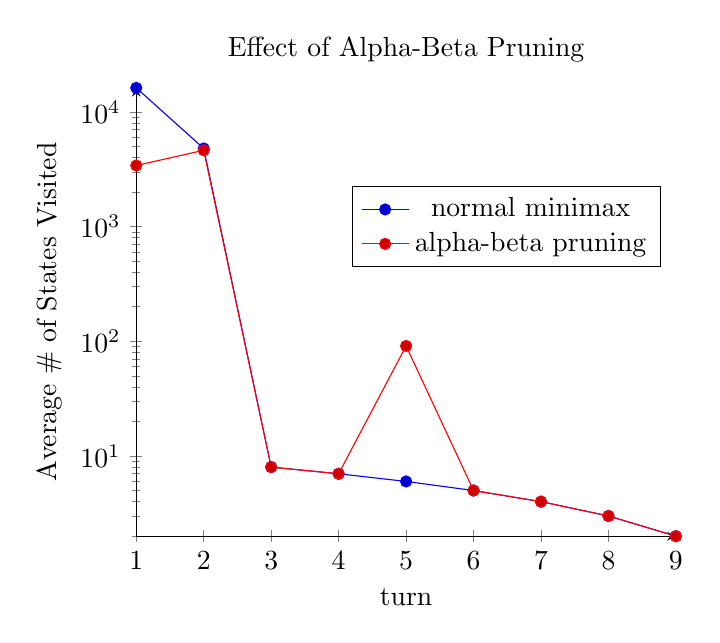
\begin{tikzpicture}
        \begin{axis}[
            legend style={at={(.4,.6)},anchor=south west},
            axis lines = left,
            xlabel = turn,
            xtick = {0, 1, 2, 3, 4, 5, 6, 7, 8, 9},
            ymode = log,
            ylabel = Average \# of States Visited,
            title = Effect of Alpha-Beta Pruning
        ]
        \addplot+[
            mark=*,
        ] plot coordinates{
            (1,16168)
            (2,4792)
            (3,8)
            (4,7)
            (5,6)
            (6,5)
            (7,4)
            (8,3)
            (9,2)
        };
        \addlegendentry{normal minimax}
        \addplot+[
            mark=*,
        ] plot coordinates{
            (1,3406)
            (2,4620)
            (3,8)
            (4,7)
            (5,91)
            (6,5)
            (7,4)
            (8,3)
            (9,2)
        };
        \addlegendentry{alpha-beta pruning}
        
        \end{axis}
    \end{tikzpicture}
\end{center}

The next graph highlights that the new hashing method (storing the hash rather than rehashing) has a consistent runtime improvment.

\begin{center}
    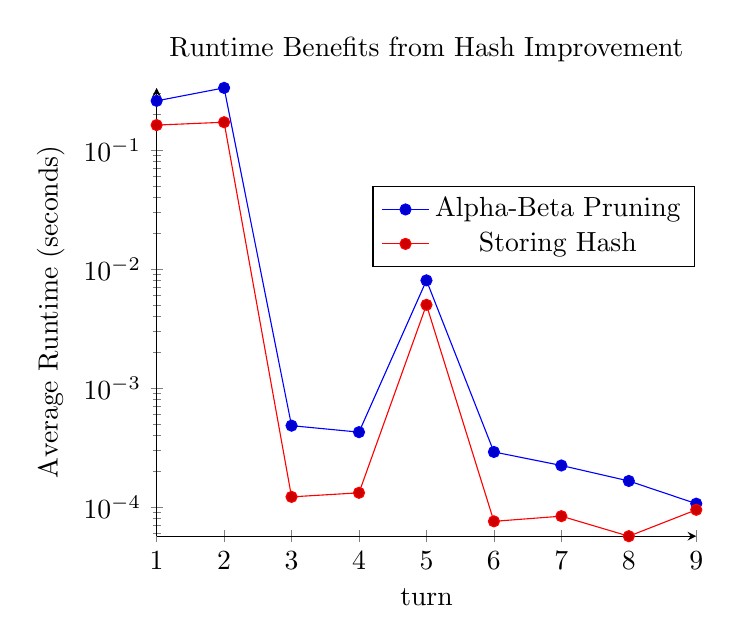
\begin{tikzpicture}
        \begin{axis}[
            legend style={at={(.4,.6)},anchor=south west},
            axis lines = left,
            xlabel = turn,
            xtick = {0, 1, 2, 3, 4, 5, 6, 7, 8, 9},
            ymode = log,
            ylabel = Average Runtime (seconds),
            title = Runtime Benefits from Hash Improvement
        ]
        \addplot+[
            mark=*,
        ] plot coordinates{
            (1,0.259692)
            (2,0.333796)
            (3,0.000484)
            (4,0.000427)
            (5,0.008052)
            (6,0.000291)
            (7,0.000224)
            (8,0.000166)
            (9,0.000107)
        };
        \addlegendentry{Alpha-Beta Pruning}
        \addplot+[
            mark=*,
        ] plot coordinates{
            (1,0.162481)
            (2,0.171736)
            (3,0.000122)
            (4,0.000132)
            (5,0.005014)
            (6,0.000076)
            (7,0.000084)
            (8,0.000057)
            (9,0.000095)
        };
        \addlegendentry{Storing Hash}
        
        \end{axis}
    \end{tikzpicture}
\end{center}

The following graph shows a comparision of states visited from a normal alpha-beta search, and two searches where moves are ordered by the current evaluation, in both a normal/positive and a reverse/negative fashion. Despite some inconsistencies, the normal move ordering seems to improve on random ordering overall (particularly on the second move), and is generally better than its reverse.
\begin{center}
    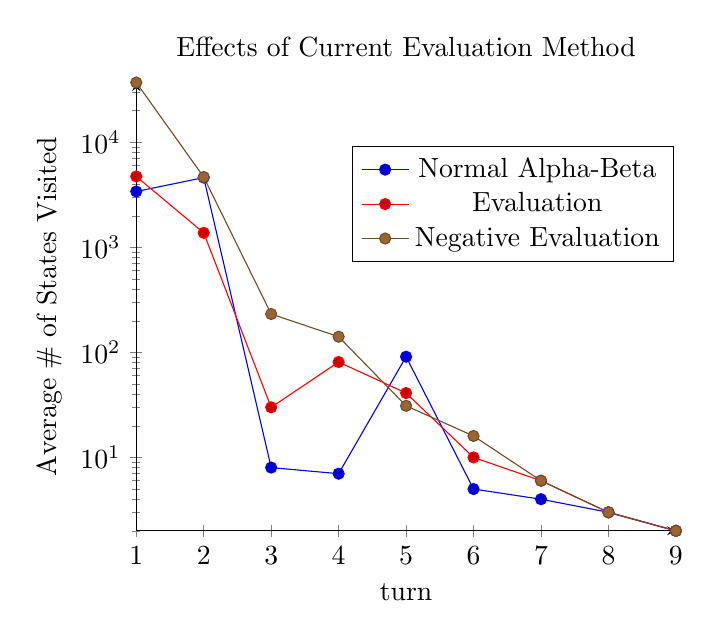
\begin{tikzpicture}
        \begin{axis}[
            legend style={at={(.4,.6)},anchor=south west},
            axis lines = left,
            xlabel = turn,
            xtick = {0, 1, 2, 3, 4, 5, 6, 7, 8, 9},
            ymode = log,
            ylabel = Average \# of States Visited,
            title = Effects of Current Evaluation Method
        ]
        \addplot+[
            mark=*,
        ] plot coordinates{
            (1,3406)
            (2,4620)
            (3,8)
            (4,7)
            (5,91)
            (6,5)
            (7,4)
            (8,3)
            (9,2)
        };
        \addlegendentry{Normal Alpha-Beta}
        \addplot+[
            mark=*,
        ] plot coordinates{
            (1,4741)
            (2,1376)
            (3,30)
            (4,81)
            (5,41)
            (6,10)
            (7,6)
            (8,3)
            (9,2)
        };
        \addlegendentry{Evaluation}
        \addplot+[
            mark=*,
        ] plot coordinates{
            (1,37182)
            (2,4675)
            (3,232)
            (4,141)
            (5,31)
            (6,16)
            (7,6)
            (8,3)
            (9,2)
        };
        \addlegendentry{Negative Evaluation}
        
        \end{axis}
    \end{tikzpicture}
\end{center}

The first couple moves clearly take up a majoirity of the runtime (by a drastic amount), so this will be the main priority when implementing further tests. Further tests on larger boards will be useful in understanding the effectiveness of move-ordering methods.

\end{document}